\section{Machine Learning based Method}




    \subsection{Naive Bayes}
        Naive Bayes is a probabilistic classification model. It is based on the Bayes theorem, which is shown in Equation \eqref{eq:bayes}:
        \begin{equation}
            \label{eq:bayes}
            P(c_j|d_i) = \frac{P(c_j) * P(d_i|c_j)}{P(d_i)}
        \end{equation}
        where $c$ is the class label and $d$ is a set of attribute values \cite{DBLP:books/aw/TanSKK2019}. 
        
        \TODO{Zitat abändern}

        Bayes theorem allows to calculate the posterior probability $P(c|d)$, which Tan et al. describe as "the probability of observing a class label $c$ for a data instance given its set of attribute values $d$" \cite[p.~418]{DBLP:books/aw/TanSKK2019}. 

        To calculate the posterior probability, the class conditional probability $P(d|c)$ is needed, which describes the probability of observing a set of attribute values given a class. One approach to calculate the class conditional probability outlined by Tan et al. is to ''consider the fraction of training instances of a given class for every possible combination of attribute values'' \cite[p.~419]{DBLP:books/aw/TanSKK2019}. With a large number of attributes and values, this method becomes computationally infeasible due to the exponential growth of combinations \cite{DBLP:books/aw/TanSKK2019}.

        Due to this, the Naive Bayes assumption is employed to estimate the class conditional probability. Naive Bayes uses conditional independence, which states that attribute values are only dependent on the class label and not each other. Thus, the class conditional probability can be calculated by using Equation \eqref{eq:naive_assumption}:
        \begin{equation}
            \label{eq:naive_assumption}
            P(d_i|c_j) = \prod_{t=1}^{n}P(w_{t}|c_j)
        \end{equation}
        with $d_i$ containing $n$ attributes $\{w_1,w_2,...,w_t\}$ \cite{DBLP:books/aw/TanSKK2019}.

        Furthermore, $P(d)$ remains constant for every class label $c$, so the class that maximizes Equation \eqref{eq:naive_final} is chosen: 
        \begin{equation}
            \label{eq:naive_final}
            P(c_j|d_i)\propto P(c_j)\prod_{t=1}^{n}P(w_{t}|c_j) 
        \end{equation}   
        
        \TODO{P(c) eingehen}
        
        There are different models on how to implement the Naive Bayes assumption for text classification. McCallum and Nigan compared two models, a multivariate Bernoulli model, and a multinomial model, and found the multinomial model to perform better at larger vocabulary sizes \cite{Mccallum1998}.
        
        According to McCallum and Nigan, "the multinomial model captures word frequency information in documents" \cite[p.~3]{Mccallum1998}. In this case, a document is represented by a tweet. By considering not only if a word is present but also how often it is present, the Bernoulli model's restriction to two values becomes uninformative. They describe the document as being "an ordered sequence of word events, drawn from the same vocabulary V" \cite[p.~3]{Mccallum1998}, with its length being independent of class. Using Naive Bayes, we assume that every word event is independent.
        
        \TODO {Gleichung?}
        
        According to Forbes et al., "the multinomial variate is a multidimensional generalization of the binomial. Consider a trial that can result in only one of $k$ possible distinct outcomes, labeled $A_i, i = 1,...,k$. The outcome $A_i$ occurs with probability $p_i$. The multinomial distribution relates to a set of n-independent trials of this type." \cite[p.~135]{evans2011statistical}.
        
        Applying this to the model, McCallum and Nigan state that "each document $d_i$ is drawn from a multinomial distribution of words with as many independent trials as the length of $d_i$" \cite[p.~3]{Mccallum1998}. Using the multinomial distribution, the class conditional probability can then be calculated using Equation \eqref{eq:multinomial_bayes}:
        \begin{equation}
            \label{eq:multinomial_bayes}
                P(d_i|c_j) = P(|d_i|)|d_i|!\prod_{t=1}^{|V|}\frac{P(w_t|c_j)^{N_{i_t}}}{N_{i_t}!}
        \end{equation}
        
        with the document $d_i$ containing $|V|$ words $w_t$, $N_{i_t}$ being the number of times $w_t$ appears in $d_i$ and $c_j$ describing a class \cite{Mccallum1998}. 
        
        To estimate $P(w_t|c_j$, the probability of a word $w_t$ given a class $c_j$, training instances are used to count the number of times a word appears in a class in Equation \eqref{eq:prob_word}:
        \begin{equation}
            \label{eq:prob_word}
                P(w_t|c_j) = \frac{1 + \sum_{i=1}^{|D|}N_{it} + P(c_j|d_i)}{|V| + \sum_{s=1}^{|V|} \sum_{i=1}^{|D|}N_{is} P (c_j|d_i)} 
        \end{equation}
        with $D$ containing labeled training documents $d_i$, $N_{it}$ describing the number of times $w_t$ appears in document $d_i$ and $|V|$ containing all words.
        Because the class conditional probabilities for labeled instances is 1 for one instance, and 0 for the other ones, Equation \eqref{eq:prob_word} can be simplified into Equation \eqref{eq:prob_word_simpler}:
                \begin{equation}
            \label{eq:prob_word_simpler}
                P(w_t|c_j) = \frac{1 + N_{tj}}{|V| + \sum_{s=1}^{|V|}N_{sj}} 
        \end{equation}
        \TODO{evtl. anderes N, erklaeren, etc.}
        
        
        with $N_{tj}$ being the number of training instances in class $c_j$ containing the word $w_t$. 
        
        By using Equation \eqref{eq:prob_word}, we calculate the word probability $P(w_t|c_j$). We utilize this in Equation \eqref{eq:multinomial_bayes} to calculate the class conditional probability $P(d_i|c_j)$ using the multinomial distribution. Finally, this allows us to estimate the posterior probability $P(c|d)$, as shown in Equation \eqref{eq:naive_final}. By selecting the class with the higher posterior probability, the classifier is able to make a prediction.
        
\subsection{Random Forest}
        According to Tan et al., Random Forest is an ensemble method that utilizes multiple base classifiers to take a vote on their predictions. The final prediction is then made by either averaging the vote or taking the majority vote. Random Forest applies a set of decorrelated decision trees by implementing two key characteristics.
        
        The first characteristic is Bagging. Each tree is trained by a data set that was sampled from the original training data. Because the sampling is done with replacement and the samples must have the same size as the original training data, the sample will, on average, only contain 63\% of the original data.
        
        The selection of input attributes is the second characteristic. When a tree is being constructed, an attribute must be selected for splitting at each internal node.
        Random Forest randomly chooses a subset of attributes, from which the attribute with the maximum reduction in an impurity measure is chosen.
        
        Through these characteristics, Random Forest reduces the correlation of trees and thus the variance \cite{DBLP:books/aw/TanSKK2019}.
        
        \begin{figure}[h!]
        \centering
        \begin{tikzpicture}
        [
        grow                    = right,
    sibling distance        = 4em,
    level distance          = 9em,
    edge from parent/.style = {draw, -latex},
    every node/.style       = {font=\footnotesize},
    sloped
  ]
  \node [root] {}
    child { node [dummy] {}
      child { node [dummy] {}
        child { node [dummy] {}
            child { node [env] {$-1.0$}
                edge from parent node [below, align=center] {$studying < 0.5$} }
            child { node [env] {$+1.0$}
                edge from parent node [above] {$studying \geq 0.5$} }
            edge from parent node [below] {$will < 0.5$} }
        child { node [env] {$-1.0$}
                edge from parent node [above] {$will \geq 0.5$} }
        edge from parent node [below] {$hates < 0.5$} }
      child { node [env] {$-1.0$}
              edge from parent node [above, align=center]
                {$hates \geq 0.5$}}
              edge from parent node [above] {$hurts \geq 0.5$} };
\end{tikzpicture}
    \caption{Part of a tree generated by the Random Forest classifier.}
      \label{fig:tree}
\end{figure}
\TODO{satzzeichen nach Gleichung, siehe Buch}
\TODO{citations}
\subsection{Logistic Regression}
Logistic Regression calculates the posterior probability $P(c_j|d_i)$ directly, without relying on the class conditional probability like Naive Bayes, which is why it is a probabilistic discriminative model. In a binary model, the class label can be assigned by calculating the odds, as seen in Equation \eqref{eq:logistic_odds}:
        \begin{equation}
            \label{eq:logistic_odds}
                \frac{P(c=1|d)}{P(c=0|d)}
        \end{equation}
If the odds are greater than 1, then the class label 1 can be assigned to document d, otherwise class 0 is assigned. Logistic Regression represents the odds using a linear predictor $z=w^Tx + b$, which results in equation \eqref{eq:logistic_linear}:
        \begin{equation}
            \label{eq:logistic_linear}
                \frac{P(c=1|d)}{P(c=0|d)} = e^z = e^{w^Td+b}
        \end{equation}
with the parameters $w$ and $b$ and $w^t$ signifying the vector transpose \cite{DBLP:books/aw/TanSKK2019}.

By substituting $P(c=0|d)$ with $1 - P(c=1|x)$ and solving for $P(c=1|d)$, we get Equation \eqref{eq:logistic_sigmoid}:
        {\begin{equation}
            \label{eq:logistic_sigmoid}
                P(c=1|d) = \frac{1}{1+e^{-z}} = \sigma(z)
        \end{equation}}
$\sigma(z)$ is called the sigmoid function, whose graph can be seen in Figure \ref{fig:sigmoid}:
        \begin{figure}[h!]
        \centering

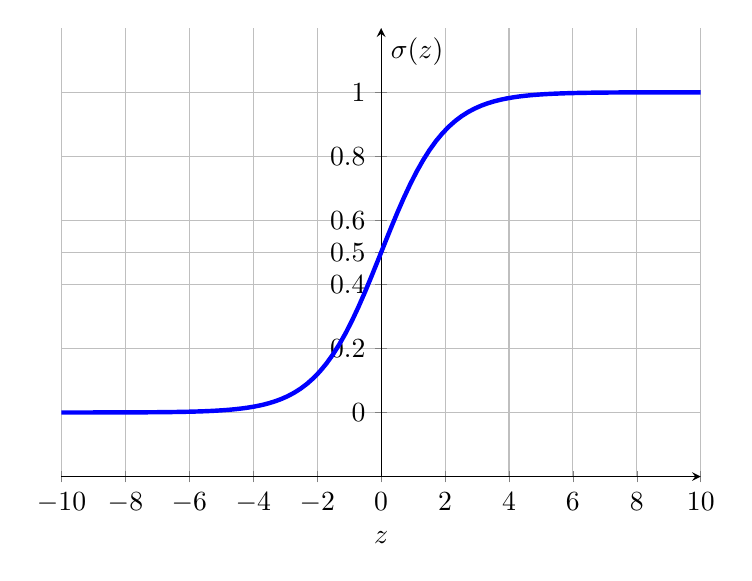
\begin{tikzpicture}
\begin{axis}
[
    grid=major,   
    xmin=-10,
    xmax=10,
    axis x line=bottom,
    ytick={0,.2,.4,.5,.6,.8,1},
    ymax=1.2,
    ymin=-0.2,
    axis y line=middle,
    width=0.8\textwidth,
    height=0.6\textwidth,
    xlabel={$z$},
    ylabel={$\sigma(z)$}
]
    \addplot%
    [
        blue,%
        mark=none,
        samples=100,
        domain=-10:10,
        ultra thick
    ]
    (x,{1/(1+exp(-x))});
\end{axis}
\end{tikzpicture}
    \caption{Plot of sigmoid function $\sigma(z)$.}
      \label{fig:sigmoid}
\end{figure}

As seen in Figure \ref{fig:sigmoid}, $\sigma(z) \geq 0.5$ when $z \geq 0$, so if $z \geq 0$, we assign the instance $d_i$ to the class $c = 1$.

Using training instances, the parameters $w$ and $b$ can be learned, and thus the posterior probability $P(c_j|d_i)$ can be estimated \cite{DBLP:books/aw/TanSKK2019}.

\subsection{Support Vector Machine}
Tan et al. describe the Support Vector Machine as a discriminative classifier. It is based on a separating hyperplane that, as the name suggests, tries to separate the instances of two classes. Furthermore, it uses a subset of the training instances, those that are the hardest to classify, meaning those nearest the boundaries of the classes. These instances are called support vectors \cite{DBLP:books/aw/TanSKK2019}.

The hyperplane can be described by Equation \eqref{eq:logistic_odds}:
    \begin{equation}
            \label{eq:logistic_odds}
                w^Td + b = 0,
        \end{equation}
    where $d$ represents the attributes and $(w, b)$ are the parameters of the model. 
    
    There can be an indefinite number of hyperplanes, which is why it is necessary to choose one that has good generalization performance, which means that it can handle unseen instances. To do this, the margin of a hyperplane $B_i$ is calculated. To achieve this, two hyperplanes, $B_i1$ and $B_i2$, parallel to $B_i$ are drawn. The distance between the two hyperplanes is the margin of the hyperplane $B_i$ \cite{DBLP:books/aw/TanSKK2019}.
    \begin{figure}
        \centering
        \caption{\TODO{source}
        \label{fig:svm}
        }
        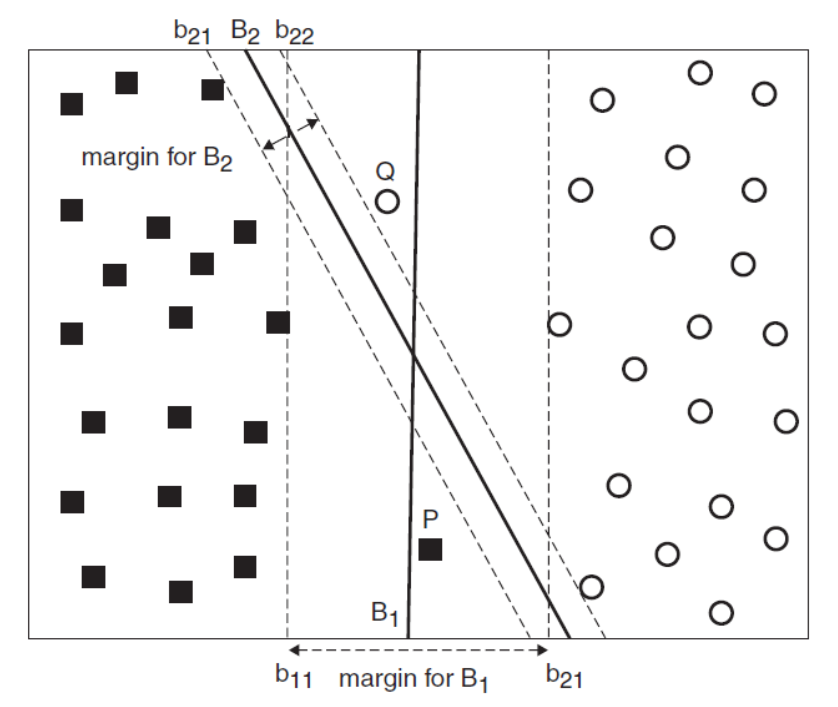
\includegraphics[scale=0.8]{Images/SVM_image.png}
    \end{figure}
    
    By choosing the hyperplane with the maximum margin, the classifier can allow for slight changes in data without immediately crossing onto the other side.
    
    In Figure \ref{fig:svm}, the data can be separated by a linear hyperplane. This is not always the case, which is why nonlinear SVM transform their input data $x$ into a new attribute space $\phi(x)$, in which a linear hyperplane can be constructed. Projected into the original attribute space, this hyperplane is a nonlinear decision boundary \cite{DBLP:books/aw/TanSKK2019}.
    
    \TODO{kernel function?}